\section{Implementering}
\label{sec:implementation}

I dette afsnit gennemgår vi implementeringsdetaljer i de funktioner som vores system består af. I flere af funktionerne har vi brugt Matlabs indbyggede funktioner, frem for at skrive egne implementeringer. For eksempel har vi brugt Matlabs funktioner i forbindelse arbejdet med sammenhængende komponenter og filtrering af billeder. I det første underafsnit gennemgår vi nogle egenudviklede hjælpefunktioner som bruges flere steder i systemet. Dernæst gennemgår vi funktionerne til lokalisering af nummerplader, separation af tegn og til sidst funktionerne til genkendelse af tegn.

Det skal bemærkes at $y$-aksen i det koordinatsystem der bruges i Matlab er vendt om i forhold til den tradionelle $y$-akse i et koordinatsystem. Desuden angives $y$-koordinaten til et punkt i Matlab først, så en pixel i et billede refereres til med koordinaterne ($y,x$) i modsætning til den traditionelle rækkefølge ($x,y$).

%Derved ligger et billedes origo i øverste venstre hjørne af billedet og er benævnt ved $(y,x) = (1,1)$ (datastrukturer i Matlab er 1-indekserede). FOR LANGT? FORKORT GERNE

%ikke har origo i det samme punkt som det man kender som et almindeligt koordinatsystem. Origo ligger derimod i øverste venstre hjørne (normalt ligger det i nederste venstre hjørne). Desuden er koordinaterne til origo i Matlab 1,1 og ikke 0,0. y-koordinaten til et punkt i Matlab angives normalt først, så en pixel i et billede refereres til med koordinaterne y,x i modsætning til den traditionelt anvendte rækkefølge x,y.

%%%%%%%%%%%%%%%%%%%%%%%%
%%% HJÆLPEFUNKTIONER %%%
%%%%%%%%%%%%%%%%%%%%%%%%

\subsection{Hjælpefunktioner}
\label{sec:imp:hjaelpefunktioner}
De følgende funktioner bruges af flere andre funktioner i systemet hvorfor vi har valgt at beskrive dem først. Vi har valgt kun et beskrive de funktioner vi finde særligt interessante. Endvidere er beskrivelsen kun overfladisk. Den specielt interesserede læser henvises til metodernes kildekode.

\subsubsection{Forstærkelse af kontrast}
\label{sec:imp:ContrastStrech}
I funktionen \textit{ContrastStretch} har vi implementeret forstærkelse af kontraster som beskrevet i afsnit \vref{sec:DetectContrastStretch} om metoden der maksimerer lokal kontrast for at lokalisere nummerplader. Funktionen tager et gråtonebillede som input og returnerer en kontrastforstærket version. 

Funktionens kildekode findes i afsnit \vref{code:ContrastStrech}

\subsubsection{Find længste lyse linie}
\label{sec:imp:GetLongestLine}
Funktionen \textit{GetLongestLine} tager et gråtonebillede som inddata og returnerer, i procent, længden af den længste lyse vandrette linie i billedet. Resultatet udregnes ved først at omdanne inddata-billedet til et binært billede, derefter findes den længste forekomst af på hinanden følgende hvide pixels i billedets rækker ved at løbe billedet igennem med en \textit{for}-løkke.  

Funktionens kildekode findes i afsnit \vref{code:GetLongestLine}

\subsubsection{Måling af intensitetsforløb}
\label{sec:imp:GetSignature}
Funktionen \textit{GetSignature} tager et gråtonebillede som inddata og returnerer en vektor der indeholder resultatet af at lægge alle intensitetsværdier i gråtonebilledets kolonner sammen. Hver plads i vektoren repræsenterer således en kolonne i billedet.

Funktionens kildekode findes i afsnit \vref{code:GetSignature}

\subsubsection{Frekvensanalyse}
\label{sec:imp:GetPlateness}
Funktionen \textit{GetPlateness} tager en vektor som returneret fra \textit{GetSignature} som inddata og returnerer et heltal. Funktionen udregner en middelværdi for inddatavektoren. Det heltal der returneres er et udtryk for hvor mange gange tallene i vektoren stiger op over og falder ned under middelværdien. Dette er illustreret på figur \vref{fig:DetectPlateness-frekvensanalyse}.

Funktionens kildekode findes i afsnit \vref{code:GetPlateness}

%%%%%%%%%%%%%%%%%%%%%%%%%%%%%%%%%%%%
%%% LOKALISERING AF NUMMERPLADER %%%
%%%%%%%%%%%%%%%%%%%%%%%%%%%%%%%%%%%%

\subsection{Lokalisering af nummerplader}
I de følgende afsnit gennemgår vi væsentlige implementeringsdetaljer i de funktioner vi bruger til lokalisering af nummerplader. De tager alle stien til et JPEG-billede som inddata og leverer koordinater til en enkelt nummerpladekandidat samt dennes point som uddata. Koordinaterne der beskriver nummerpladekandidatens position i inddata-billedet angives i rækkefølgen: Mindste \textit{x}-værdi, største \textit{x}-værdi, mindste \textit{y}-værdi og største \textit{y}-værdi. Hvis en funktion ikke kan finde en nummerpladekandidat returneres et koordinatsæt, hvor alle værdier er $0$.

I metoderne til lokalisering af nummerplader nedskalerer vi billederne til en fjerdedel. Det vil sige at opløsningen bliver $256 \times 192$ pixels i stedet for $1024 \times 768$ pixels. Den lavere opløsning gør billederne langt hurtigere at arbejde med. Da vi ikke arbejder med analyse af teksten på nummerpladen i disse metoder, men blot forsøger at udpege områder der indeholder nummerplader, bekymrer vi os ikke om hvorvidt nummerpladens tegn kan læses i billeder med denne lave opløsning.

Ofte udvider vi kandidatområdet før vi returnerer det for at få hele pladen med. Det er vigtigt for at senere at kunne rotere, da dette kræver tilstædeværelsen af markante linier, der markerer pladens over- og underkant. Vi vil hellere returnere områder der er lidt for store, end områder der er lidt for små.



\subsubsection{Analyse af interesseområder}
\label{sec:imp:BinImgCleanup}
Funktionen der fjerner områder vi opfatter som uinteressante i de binære billeder der markerer interesseområder, varetages af funktionen \textit{BinImgCleanup} hvis kildekode findes i afsnit \vref{code:BinImgCleanup}. Denne funktion bliver brugt af alle de fem metoder vi bruger til at lokalisere nummerplader.

Funktionen tager et binært billede samt en skaleringsværdi som inddata og returner et binært billede, hvor de områder der sandsynligvis ikke er nummerpladeområder er fjernet, som beskrevet i afsnit \vref{sec:BinImgCleanup}.

Det er nødvendigt at angive en skaleringsværdi, da vi i programmet har defineret hvor høje og brede nummerplader maksimalt må være som heltalsvariable. Da disse værdier er baseret på analyse af billeder med en opløsning på $1024 \times 768$ pixels har vi behov for at gøre disse variable mindre når man arbejder på billeder med en lavere opløsning. Hvis man for eksempel giver funktionen et binært billede med en opløsning på $512 \times 384$, skal skaleringsværdien være $0.50$, da billedets højde og bredde er halvt så store, hvorimod den skal være $1.0$, hvis opløsningen er $1024 \times 768$, da variablene ikke skal ændres og derfor ganges med 1.

Behandlingen af det binære billede foregår i de følgende trin:

\paragraph{1. Udregn sammenhængende komponenter:}
Med Matlabs funktion \textit{bwlabel} udregner og nummererer vi de sammenhængende komponenter i inddatabilledet. Vi opfatter pixels der ligger direkte ved siden af hinanden eller over hinanden som værende sammenhængende. Øvrige pixels opfatter vi som selvstændige områder. Figur \vref{fig:con_comp-connections} illustrerer disse forhold.

BEDRE ILLU

\begin{figure}[htp]
\centering

\includegraphics[width=7cm]{implementation/illu/con_comp-connections.jpg}
\caption{De fem pixels i figuren til venstre opfatter vi som ét sammenhængende område, mens vi opfatter de fem pixels i figuren til højre som fem forskellige områder.}
\label{fig:con_comp-connections}
\end{figure}

\paragraph{2. Analyser størrelser:}
Vi sletter alle områder, der er for store eller for små i forhold til de størrelser på nummerplader vi har observeret i vores træningssæt.

\paragraph{3. Analyser forholdet mellem bredde og højde:}
Vi sletter alle områder hvor højden er større end den halve bredde, det vil sige kvadrater og stående rektangler, eller hvor bredden er større end højden ganget med 7, det vil sige meget flade liggende rektangler. Vi sletter altså de områder, hvis bredde/højde-forhold adskiller sig væsentligt fra de nummerplader vi søger.

\paragraph{4. Analyser densitet:}
For hvert interesseområde kigger vi på det rektangel det udspænder. Hvis interesseområdet udgør mindre end en tredjedel af rektanglet sletter vi det, da vi forventer en højere densitet i vores nummerpladeområder.

\paragraph{5. Returner binært billede:}
Vi bruger Matlabs funktion \textit{im2bw} for at skabe det binære billede vi returnerer på baggrund af de tilbageværende sammenhængende komponenter. 

%%%%%%%%%%%%%%%%%%%%
\subsubsection{Valg af bedste nummerpladekandidat}
\label{sec:imp:GetBestCandidate}
Programmet der udvælger den bedste nummerpladekandidat er implementeret i funktionen \textit{GetBestCandidate2} hvis kildekode findes i afsnit \vref{code:GetBestCandidate2}. Funktionen tager en liste med sammenhængende komponenter, et gråtonebillede og den skaleringsfaktor der er anvendt på gråtonebilledet som argumenter og returnerer den bedste nummerpladekandidats point samt dens koordinater, som de er i et billede med en opløsning på $1024 \times 768$. Billeder af nummerplader, der er skåret helt tæt til, opnår omkring 60-70 point. Områder der får under 100 point er gode nummerpladekandidater. 

Pointgivningen sker ved at måle nummerpladekandidaternes afvigelser i forhold til optimale værdier for en række karakteristika for nummerpladeområder som tidligere beskrevet i afsnit \vref{sec:GetBestCandidate}.
Programmet udfører følgende trin:

\paragraph{1. Tildel point:}
En løkke analyserer nummerpladekandidaterne og udregner deres point for hver af de karakteristika vi analyserer. Vi lægger pointene sammen for at finde nummerpladekandidaternes endelige point. For at udregne point på baggrund af frekvensanalyse af nummerpladekandidaterne bruger vi hjælpefunktionerne \textit{GetSignature} og \textit{GetPlateness}, der begge er beskrevet i det tidligere afsnit \vref{sec:imp:hjaelpefunktioner}. 

\paragraph{2. Returner den bedste nummerpladekandidat:}
Vi returnerer koordinater og point for den nummerpladekandidat med det laveste antal point. Hvis der ikke findes en kandidat med mindre end 300 point, signalerer vi, at der ikke kunne findes en nummerplade ved at returnere koordinaterne $(0,0,0,0)$ 


%%%%%%%%%%%%%%%%%%%%%%
\subsubsection{Metode: Områder domineret af lyse gråtoner}
Metoden hvor vi førsøger at finde nummerplader ved at kigge på grå områder i farvebilleder er implementeret i funktionen \textit{DetectSameness} hvis kildekode findes i afsnit \vref{code:DetectSameness}. Funktionens eneste argument er stien til et farvebillede i JPEG-format i en opløsning på $1024 \times 768$ pixels. Programmet udfører følgende trin:

\paragraph{1. Klargør originalbillede:}
Billedet indlæses og nedskaleres til en fjerdedel. 

\paragraph{2. Skab binært billede:}
På baggrund af formlen i afsnit \ref{sec:DetectSameness} danner vi et binært billede hvor de områder hvor lysere gråtoner dominerer i originalbilledet er markeret.

\paragraph{3. Manipuler binært billede:}
For at forsøge at undgår at nummerpladeområdet er forbundet med andre områder, trækker vi alle områder i det binære billede en anelse sammen. Vi bruger Matlabs funktion \textit{imerode} med et kvadrat på $2 \times 2$ pixels som figur. Dette trin kan muligvis have delt nummerpladeområdet op i flere områder. For igen at have et samlet nummerpladeområde, udvidder vi alle områder i det binære billede med Matlabs \textit{imdilate}-funktion. Denne gang bruger vi et liggende rektangel med højden 2 og bredden 4 som figur. Vi bruger denne liggende figur, da vi ønsker at forbinde områder som ligger ved siden af hinanden, dele af nummerpladen, men vil undgå at forbinde områder der ligger over og under hinanden. 

OVERVEJ ILLU FRA: http://www.ph.tn.tudelft.nl/Courses/FIP/noframes/fip-Morpholo.html

\paragraph{4. Fjern uinteressante områder fra binært billede:}
I det binære billede er der nu en masse områder, som helt sikkert ikke kan være nummerpladen. Et helt oplagt eksempel er områder der kun består af ganske få pixels. Vi sletter alle de områder vi vurderer som uinteressant ved at kalde funktionen \textit{BinImgCleanup} som tidligere beskrevet i \vref{sec:imp:BinImgCleanup} med det binære billede som argument.

\paragraph{5. Vælg den bedste nummerpladekandidat:}
For at finde den bedste nummerpladekandidat i det nu ``rensede'' binære billede kalder vi funktionen \textit{GetBestCandidate} som tidligere beskrevet i afsnit \vref{sec:imp:GetBestCandidate}. Funktionen returnerer koordinater og point for den nummerpladekandidat, der har fået færrest point. 

\paragraph{6. Returner resultat:}
For at forsøge at sikre os at koordinaterne dækker hele nummerpladeområdet, udvidder vi området en smule før vi returnerer det og de tilhørende point fra det foregående trin. 


%%%%%%%%%%%%%%%%%%%%%%%%%%%%%%%%%%%%%%%%%%
\subsubsection{Metode: Områder med høj kontrast}
Metoden hvor vi forsøger at finde nummerplader ved at markere områder med høj kontrast er implementeret i funktionen \textit{DetectContrastAvg} hvis kildekode findes i afsnit \vref{code:DetectContrastAvg}. Funktionens eneste argument er stien til et farvebillede i JPEG-format i en opløsning på $1024 \times 768$ pixels. Programmet udfører følgende trin:

\paragraph{1. Klargør originalbillede:}
Billedet indlæses og konverteres fra \textit{RGB} til 256 gråtoner. Herefter nedskaleres det til en fjerdedel. DER ER LOG I KODEN. VI GØR BILLEDET LYSERE. BESKRIV!

\paragraph{2. Udregn gradienter:}
Vi udregner gradienterne for gråtonebilledet med Matlabs kommando \textit{gradient}. Herefter finder vi gradienternes længder og deres vinkler målt som forskel til vandret. Det vil sige at gradtallet går fra $0^\circ$ til $90^\circ$ og så til $0^\circ$ igen. Vi normaliserer gradienternes længder til $1$ og danner et nyt billede bestående af de gradienter der har en vinkel med det vandrette plan på mellem $0^\circ$ og $30^\circ$. Hvis en gradient har en størrelse på $0.25$ eller mere, fordobler vi den værdi der sættes ind. Vi giver altså de største gradienter, svarende til områder med høj kontrast, mere vægt i billedet. De pixels der svarer til de øvrige gradienter i originalbilledet får værdien $0$ i det nye billede. Et eksempel på dette billede er vist i figur \vref{fig:DetectContrastAvg-hgrads}.

\paragraph{3. Filtrer billedet:}
For at forsøge at forbinde de mange markeringer i nummerpladeområdet som vist i figur \vref{fig:DetectContrastAvg-blurredGrads} filtrerer vi billedet. Filteret udregner gennemsnitsværdien for hver pixels nærområde og giver den indeværende pixel 80\% af denne værdi som foreslået af \cite{shapiro}. Da vi kun ønsker at forbinde områder der ligger ved siden af hinanden anvender vi et filter, der er 3 pixels højt og 7 pixels bredt. Vi anvender Matlabs funktion \textit{nlfilter} for at foretage filtreringen.

\paragraph{4. Lav binært billede:}
På baggrund af det filtrerede billede danner vi et binært billede. Som grænseværdi bruger vi halvdelen af resultatet af Matlabs funktion \textit{graythresh}. På denne måde får vi større, mere sammenhængende, områder i det binære billede end dem vi ville have fået hvis vi direkte havde benyttet resultatet af \textit{graythresh}.

\paragraph{5. Fjern uniteressante områder fra binært billede:}
Vi sletter de områder vi vurderer som uinteressante i det binære billede ved at kalde funktionen \textit{BinImgCleanup}.

\paragraph{6. Vælg den bedste nummerpladekandidat}
For at finde den bedste nummerpladekandidat i det nu ``rensede'' binære billede kalder vi funktionen \textit{GetBestCandidate} som returnerer koordinater og point for den bedste nummerpladekoordinat.

\paragraph{7. Returner resultat}
De nummerpladekandidater der rent faktisk indeholder nummerplader, bliver fladere end pladen rent faktisk er, da der jo ikke er nogle stærke kontraster over og under nummerpladernes tekst og disse områder derfor ikke bliver markeret. For at forsøge at få hele pladen med, udvider vi kandidaten med 15 pixels på over- og underkanten. 

%%%%%%%%%%%%%%%%%%%%%%%%
\subsubsection{Metode: Frekvensanalyse}
Metoden hvor vi forsøger at finde nummerplader ved at markere områder på baggrund af frekvensanalyse er implementeret i funktionen \textit{DetectPlateness}, hvis kildekode findes i afsnit \vref{code:DetectPlateness}. Funktionens eneste argument er stien til et farvebillede i JPEG-format i en opløsning på $1024 \times 768$ pixels. Programmet udfører følgende trin:

\paragraph{1. Klargør originalbillede:}
Billedet indlæses og konverteres fra \textit{RGB} til 256 gråtoner. Herefter nedskaleres det til en fjerdedel.

\paragraph{2. Frekvensanalyse:}
Vi filtrerer billedet ved at for hver pixel i originalbilledet at kigge på rækken af pixels startende fra 11 pixels før den indeværende pixel til den 11. pixel efter. Vi kigger altså på et udsnit af originalbilledet der er 1 pixel højt og 23 pixels bredt\footnote{Bredden ville have været anderledes hvis man havde valgt en anden nedskalering end $0.25$.}. Med et kald til funktionen \textit{GetPlateness} får vi et tal, der beskriver svingninger mellem lyse og mørke områder i billedudsnittet. Vi udregner forskellen mellem dette tal og den gennemsnitlige frekvens for nummerpladeområder som observeret i vores testsæt. I det filtrerede billede bliver intensiteten på den indeværende pixels position denne forskel. Filteret er implementeret i en dobbelt \textit{for}-løkke.

Da filteret ikke er defineret for de første og sidste 11 pixels i billedets linier\footnote{Der er for eksempel ikke 11 pixels til venstre for den første pixel i billedets linier, ligesom der ikke er 11 pixels til højre for den sidste pixel i en linie i billedet.}, vil denne metode ikke kunne lokalisere nummerplader der er ``i kontakt'' med disse områder.

HVORFOR 11 PIXELS

\paragraph{3. Lav binært billede:}
Med en grænseværdi udregnet af Matlabs \textit{graythresh}-funktion laver vi et binært billede på baggrund af det filtrerede område. Da de områder vi er interesserede i har værdier der er meget tæt på 0, det vil sige de adskiller sig meget lidt fra den ideelle frekvens, inverterer vi det binære billede så interesseområderne bliver de hvide markerede områder. 

\paragraph{4. Fjern uniteressante områder fra binært billede:}
Vi sletter de områder vi vurderer som uinteresante i det binære billede ved at kalde funktionen \textit{BinImgCleanup}.

\paragraph{5. Vælg den bedste nummerpladekandidat:}
Vi finde den bedste nummerpladekandidat i det binære billede med et kald til funktionen \textit{GetBestCandidate} som returnerer koordinater og point for den bedste nummerpladekoordinat.

\paragraph{6. Returner resultat:}
Da vi ved frekvensanalysen ikke får de hvide områder over og under nummerpladens tegn markeret, udvider vi kandidatområdet i højden før det returneres med de tilhørende point som udregnet i det foregående trin.


%%%%%%%%%%%%%%%%%
\subsubsection{Metode: Maksimer lokal kontrast}
Metoden hvor vi førsøger at finde nummerplader ved at maksimere lokal kontrast er implementeret i funktionen \textit{DetectCStretch} hvis kildekode findes i afsnit \vref{code:DetectCStretch}. Funktionens eneste argument er stien til et farvebillede i JPEG-format i en opløsning på $1024 \times 768$ pixels. Programmet udfører følgende trin:

\paragraph{1. Klargør originalbillede:}
Billedet indlæses, konverteres til gråtoner og nedskaleres til en fjerdedel. 

\paragraph{2. Maksimer lokal kontrast:}
For hvert kvadrat af $4 \times 4$ pixels i gråtonebilledet maksimerer vi kontrasten ved at kalde den i afsnit \vref{sec:imp:ContrastStretch} beskrevne funktion \textit{ContrastStrech}.

\paragraph{3. Skab binært billede:}
På baggrund af billedet dannet i det foregående trin danner vi et binært billede. Som grænseværdi benytter vi resultatet af Matlabs \textit{graythresh}-funktion ganget med $1.2$. Vi gør grænseværdien højere for at gøre de markerede områder i det binære område mindre og dermed gøred det mindre sandsynligt at nummerpladeområdet er forbundet med andre områder.

\paragraph{4. Fjern uinteressante områder fra binært billede:}
Vi sletter de uinteresante områder i det binære billede med et kald til funktionen \textit{BinImgCleanup}.

\paragraph{5.Vælg den bedste nummerpladekandidat:}
Vi får koordinater og point for den bedste nummerpladekandididat i det binære område ved at kalde funktionen \textit{GetBestCandidate}. 

\paragraph{6. Returner resultat:}
Vi udvider nummerpladekandidaten en smule i alle retninger før den returneres med tilhørende point.

%%%%%%%%%%%%%%%%%%%%%%%%
\subsubsection{Metode: Kvantifisering}
Metoden hvor vi førsøger at finde nummerplader ved at sætte antallet af gråtoner i billederne meget kraftigt ned, er implementeret i funktionen \textit{DetectQuant} hvis kildekode findes i afsnit \vref{code:DetectQuant}. Funktionens eneste argument er stien til et farvebillede i \textit{JPG}-format i en opløsning på $1024 \times 768$ pixels. Programmet udfører følgende trin:

\paragraph{1. Klargør originalbillede:}
Billedet indlæses, konverteres til gråtoner og nedskaleres til en fjerdedel. 

\paragraph{2. Filtrer billede:}
For at skabe et tilnærmelsesvis ensfarvet sammenhængende rektangel, der hvor nummerpladen er, udvisker vi tegnene i nummerpladen ved at filtrere billedet. Vi anvender et filter der for hver pixel i billedet kigger på nærområdet og finder den lyseste pixel. Hver pixels sættes til denne lokale maksimale intensitet. Formen på filtet er et rektangel med højden 5 pixels og bredden 7 pixels. Vi vælger en større bredde end højde i et forsøg på at give filteret mere af  nummerpladen at arbejde med. Havde filteret været et lodret rektangel ville det være mere sandsynligt at de maksimale intensiteter i nærområdet for pixels i nummerpladeområdet ville stamme fra andre områder end nummerpladen.

\paragraph{3. Sæt antal gråtoner ned:}
Vi dividerer alle intensiteter i det filtrerede billede med $37$, runder af og lægger 1 til. På den måde indeholder billedet nu kun intensiteter mellem 1 og 8. De 8 intensiteter skaber nu større sammenhængende områder.  

\paragraph{4. Skab binært billede:}
For hver af de 8 intensiteter skaber vi et binært billede hvor kun de pixels med netop den intensitet er markerede. Vi fjerner uinteressante områder i hver af disse 8 billeder med funktionen \textit{BinImgCleanup}. Herefter slår vi de 8 ``rensede'' binære billeder sammen til et enkelt. Hvis områder i billede ligger helt op til hinanden bliver de nu til større sammenhængende områder. Man kunne også her have valgt at trække områderne i de 8 binære billeder en smule sammen før sammenlægningen for at undgå at de kommet til at hænge sammen. Vores erfaring er at det giver de bedste resultater at lade områderne flyde sammen.   

\paragraph{5. Fjern uniteressante områder fra binært billede:}
Vi benytter igen funktionen \textit{BinImgCleanup} til at fjerne områder i det binære billede vi vurderer som uinteressante efter en analyse af deres størrelser og bredde/højde forhold.

\paragraph{6. Vælg den bedste nummerpladekandidat:}
Vi får koordinater og point for den bedste nummerpladekandididat i det binære område ved at kalde funktionen \textit{GetBestCandidate}. 

\paragraph{7. Returner resultat:}
Vi udvider nummerpladekandidaten en smule i alle retninger før den returneres med tilhørende point.

%%%%%%%%%%%%%%%%%%%%%%%%%%%%%%%%%%%%
\subsubsection{Endeligt valg af nummerpladekandidat}
Funktionen der sammenligner resultaterne for samtlige metoder til lokalisering af nummerplader er implementeret i funktionen \textit{DetectMain} hvis kildekode findes i afsnit \vref{code:DetectMain}. Funktionen tager stien til et farvebillede i en opløsning på $1024 \times 768$ lagret som en JPEG-fil som argument og returnerer koordinater til nummerpladen i billedet. Hvis funktionen ikke kan lokalisere en nummerplade i billedet returnerer den koordinaterne $(0,0,0,0)$. Funktionen udfører følgende trin: 

\paragraph{1. Kald metoder lokalisering af nummerplader:}
Vi kalder de fem metoder til lokalisering af nummerplader og modtager koordinater og point for hver metodes nummerpladekandidat. Vi ignorerer svaret fra metoder der returnerer koordinaterne $(0,0,0,0)$ som indikation på at en nummerpladekandidat ikke kunne findes.

\paragraph{2. Afgør eventuel enighed om nummerpladekandidater:}
Vi undersøger om flere metoder har udpeget de samme områder. For hver nummerpladekandidat ser vi om dens centrum ligger inden for de midterste 80\% af andre nummerpladekandidater for at afgøre, om de er enige om det samme område. Figur \vref{fig:enighed} illustrerer dette princip.

\begin{figure}[htp]
\centering
\includegraphics[width=8cm]{implementation/illu/illu_enighed.png}
\caption{Enighed blandt nummerpladekandidater: Nummerpladekandidat \textbf{A} er enig med nummerpladekandidat \textbf{B} da dens centrum \textbf{a} ligger inde i \textbf{B}s midterste område som indikeret af den stiplede linie. \textbf{C} er uenig med \textbf{D} da dens centrum \textbf{c} ligger uden for \textbf{D}s midterste område.}
\label{fig:enighed}
\end{figure}

\paragraph{3. Vælg den endelige nummerpladekandidat:}
Vi kigger på omfanget af enighed blandt de udpegede nummerpladekandidater. Niveauet af enighed kan være mellem et og fem. Hvis tre eller flere metoder er enige returnerer vi den nummerpladekandidat de er enige om. Hvis niveauet af enighed er to, er der to mulige situationer. Den ene er, at to metoder har udpeget et område mens to andre metoder har udpeget et andet. I dette tilfælde udregner vi gennemsnitspointene for hver gruppe af enige områder, og returnerer det område med lavest point som nummerplade. Den anden mulighed er at der kun er et område som to metoder er enige om. I dette tilfælde returnerer vi det område uden yderligere overvejelser. Hvis niveauet af enighed er et, er situationen enten at flere metoder har udpeget forskellige områder, eller at kun en enkelt af de fem metoder har returneret en nummerpladekandidat. I disse situationer kigger vi på hver nummerpladekandidats antal point. Vi returnerer den kandidat med lavest antal point, såfremt dette er under 100. Har alle kandidater mere end 100 point returnerer vi ingen nummerplade for det aktuelle billede.

%%%%%%%%%%%%%%%%%%%%%%%%%%%%%%%%%%%%%
\subsubsection{Mulige forbedringer}
Vi kunne arbejde mere med manipulation af de binære billeder før vi renser dem. Vi kunne arbejde mere med støjfiltrering etc. altså preprocessing af billederne. Citer folk der gør det. Skriv også hvad de gør.
Man kunne have taget højde for at de forskelleige metoder returnerer områder af forskellig bredde og intensitet.

Mere tuning af vægte etc i pointsystem. Arbejde med kriterier der skal vær opfyld. Vis nogle billeder fra kontrolsættet som er blevet valgt som kandidater men tydeligvis, visuelt, ligger langt fra noget man ville forveksle med en nummerplade. Mere skrap med enighed.


DetectPlateness:
Metoden bliver dårligere jo mere man skalerer billedet ned da tegn i nummerpladerne ikke længere er klart separeret. Vi burde nok køre dette på større billeder.
Vi bruger funktionen plateness. Den kunne være mere robust.

Lokal contrast stretch:
Måske kunne vi opnå bedre resultater ved at bruge filter frem for blok, men blok er meget hurtigere.

DetectMain: Der er fejl i 2x2 situationer.


%%%%%%%%%%%%%%%%%%%%%%%%%%
%%% SEPARATION AF TEGN %%%
%%%%%%%%%%%%%%%%%%%%%%%%%%

\subsection{Separation af tegn}

I de følgende afsnit gennemgår vi væsentlige implementeringsdetaljer i de funktioner vi bruger til separation af tegn.

\subsubsection{Rotation}
\label{sec:implementation/sep/rotation}

I dette afsnit vil vi gennemgå funktionen der roterer et billede ved brug af Radon transformation. Vi vil dog undlade at gennemgå definitionen af denne transformation, da vi ikke mener det er væsentligt i denne forbindelse.

Metoden til rotation er implementeret i funktionen \textit{RotatePlateRadon}, hvis kildekode findes i afsnit \vref{code:RotatePlateRadon}. Metoden tager stien til et JPEG-billede samt koordinaterne for nummerpladen i billedet som inddata. Funktionen returnerer billedet af den roterede plade samt dennes (roterede) koordinater i originalbilledet. Funktionens forløb er som følger:

\paragraph{1. Skær billedet af nummerpladen ud af originalbilledet:}
Nummerpladen findes ved hjælp af pladekoordinaterne, der er returneret fra lokaliseringsmetoderne.

\paragraph{2. Find vandrette kanter i billedet:}
For at finde pladens rotation er det nødvendigt at finde kanterne i billedet af nummerpladen. Matlab funktionen \textit{edge} bruges til at lave et binært billede hvor alle kanter er markeret. Vi undlader dog at markere de vertikale kanter. På denne måde kan vi nøjes med at analysere kanter i tilnærmelsesvis horisontal retning ved brug af Radon transformationen. Vi er interesserede i de kanter, der er (næsten) horisontale, da det med stor sandsynlighed er de liggende kanter som spænder i nummerpladens bredde. Det vil være et problem, hvis nummerpladen udklippes så tæt at den øvre eller nedre kant af nummerpladen ikke kommer med i billedet. I dette tilfælde er det usikkert om de horisontale kanter i nummerpladens tegn vil være kraftige nok til, at Radon transformationen vil opfatte en af disse kanter som den tydeligste kant.

VIS EKSEMPEL MED AT DEN IKKE KAN ROTERERE HVOR PLADEN ER KLIPPET FOR TÆT. SKAL DETTE VISES?

\paragraph{3. Udfør Radon transformation for kant-billedet:} Radon transformation udføres ved brug af Matlab funktionen \textit{radon}.

\paragraph{4. Find den maksimale værdi i Radon matricen:} Den maksimale værdi i Radon matricen svarer til det sted i billedet, hvor den tydeligste linie findes. De polære koordinater (afstand samt vinkel) for linien aflæses, men kun vinklen, $\theta$ bruges i den videre analyse. \textit{radon} funktionen angiver vinklerne forskudt med $90^{\circ}$ i forhold til det normale, så rotationsvinklen beregnes som $90^{\circ} - \theta$.

\paragraph{5. Roter billedet af nummerpladen:} Rotationen foretages ved hjælp af funktionen \textit{imrotate} med pladens midte som omdrejningspunkt.

\paragraph{6. Koordinaterne til den roterede plade findes ved brug af en rotationsmatrix:} Vi roterer de to todimensionale koordinatsæt ved hjælp af en rotationsmatrix, \textit{R} der er defineret således:
%, $P=\biggl[\begin{array}{c} x\\ y\\ \end{array}\biggr]$
\begin{displaymath} 
R = 
\biggl[ \begin{array}{cc} 
\cos(\theta) & - \sin(\theta) \\
\sin(\theta) & \cos(\theta) \\
\end{array} \biggr] 
\end{displaymath}

Hvert koordinatsæt der repræsenteres ved en vektor, $\biggl[\begin{array}{c} x\\ y\\ \end{array}\biggr]$ roteres ved at gange vektoren med $R$.

\paragraph{7. Returner det roterede billede og de roterede koordinater:} HVAD KAN STÅ HER?

\subsubsection{Separation}

Metoderne til separation af tegn tager et billede af en nummerplade samt koordinaterne til denne plade i orginalbilledet som inddata, og returnerer syv billeder af de syv tegn (hvis syv tegn er fundet), koordinaterne til disse tegn i originalbilledet samt antallet af fundne tegn som uddata.

\subsubsection*{Sammenhængende komponenter}

Denne metode er implementeret i funktionen \textit{CharSeparationCC}, hvis kildekode findes i afsnit \vref{code:CharSeparationCC}. Programmet forløber således:

\paragraph{1. Klargør billedet:} Billedet af pladen omdannes fra RGB til 256 gråtoner.

\paragraph{2. Indskrænk billedet til den største komponent:}
De billeder der i denne del af systemet modtages fra lokaliseringsmetoderne er ikke nødvendigvis udskåret så nøjagtigt at nummerpladen dækker hele billedet. Billedet kan derfor indeholde elementer som ikke er en del af nummerpladen (eksempelvis et klistermærke som sidder på bilen). Derfor er det hensigtsmæssigt, når tegnene i nummerpladen skal separeres, at indskrænke billedet så det mest muligt kun forestiller nummerpladen. Vi kan desuden antage flere ting om billedet, når vi ved, at det kun indeholder pladen. Da nummerpladen sandsynligvis er det mest lyse element i billedet, indskrænker vi ved at gøre billedet binært og indskrænke det til det største hvide område i billedet. Billedet gøres binært ved hjælp af Matlab funktionen \textit{im2bw}, hvor grænsen for hvilke intensitetsværdier der skal være markerede i det binære billede sættes under middel. Ved at sætte denne grænseværdi lavt mindskes risikoen for at nummerpladen ikke bliver et samlet element i det binære billede.

\paragraph{3. Forstærk billedets kontraster:}
For at få nummerpladens tegn til at adskille sig mest muligt fra pladens hvide baggrund kontrastforstærkes billedet. Her bruges hjælpefunktionen \textit{ContrastStretch}. Denne funktion udføres i mindre blokke i billedet ved hjælp af Matlab funktionen \textit{nlfilter}. Ved at udføre operationen i blokke vil man udover den forstærkede kontrast mellem tegnene og baggrunden også opnå forstærket kontrast mellem støj (for eksempel urenheder i nummerpladen) og baggrunden. Hvis denne støj er tæt på et tegn vil der være chance for at tegnet ``gror'' sammen med støjen og derfor bliver sorteret fra når de sammenhængende komponenter analyseres. Hvis kontrasten forstærkes i blokke, er der dog en mulighed for at støjen og tegnets kant vil blive adskilt. Størrelsen af blokkene der arbejdes med har vi bestemt eksperimentielt.

HER ER BRUG FOR EN ILLUSTRATION. ER DER VIRKELIG? :)

\paragraph{4. Omdan billedet til et binært billede:} Billedet gøres binært ved hjælp af Matlab funktionen \textit{im2bw}.

\paragraph{5. Fjern smalle elementer i toppen og i siderne af billedet:}
Når det binære billede er dannet, er der igen en mulighed for at minimere antallet af tilfælde, hvor tegn er groet sammen med eksempelvis nummerpladens kant. I nogle tilfælde gror to elementer sammen med en smal ``bro''. Dette er illustreret i figur \vref{fig:tynd_linie}. Derfor slettes alle pixels som har en tom plads på begge sider i den øverste $\frac{1}{3}$ af billedet, samt i den yderste $\frac{1}{10}$ i både højre og venstre side. Grunden til at det også gøres i yderkanterne af billedet er at det ``brækker'' tynde elementer over, som på grund af deres højde kan forveksles med tegn i den senere analyse. Det er dog en dårlig idé at brække tynde elementer over i hele billedet, da der så er chance for at nogle af tegnene brækkes over (eksempelvis er tegnet \textbf{1} smalt) og derfor ikke længere vil være et sammenhængende element.

\begin{figure}[htp]
\centering
\includegraphics{implementation/illu/cc_remove_thin_line.png} 
\caption{En illustration af hvordan to hvide elementer kan gro sammen med en smal bro. Det øverste hvide område (over den grå pixel) er eksempelvis nummerpladens kant mens det nederste hvide område eksempelvis er et tegn. Det sorte er baggrund. Den grå pixel illustrerer et punkt hvor de to hvide elementer er groet sammen (den grå pixel er i virkeligheden hvid).}
\label{fig:tynd_linie}
\end{figure}

\paragraph{5. Fjern al markering i meget eller lidt hvide horisontale linier:} En horisontal linie der går igennem tegnene i en nummerplade vil have mellem $\frac{1}{10}$ og $\frac{2}{3}$ af linien markeret. Derfor kan vi slette alle pixels i de rækker af billedet, som har mindre end $\frac{1}{10}$ eller mere end $\frac{2}{3}$ af alle pixels i billedets bredde markeret. Dette vil fjerne flere muligheder for at tegn og pladens kant kan gro sammen. Man kunne overveje at gøre det i den vertikale retning, men vores undersøgelser viste at dette ofte skærer tegnet \textbf{K} over, da det er meget smalt i midten.

VIS SITUATIONEN PÅ EN ILLU?

\paragraph{6. Lav det sort-hvide billede til sammenhængende-komponenter-billede:} Sammenhængende komponenter udregnes og nummereres ved brug af Matlab funktionen \textit{bwlabel}. I modsætning til illustrationen i figur \vref{fig:con_comp-connections} vælger vi her, at sammenhængende komponenter består af pixels der støder op til hinanden vandret og lodret men også diagonalt. På denne måde sikrer vi os, at tegn der har diagonale/skæve sider også bliver en sammenhængende komponent.

\paragraph{7. Fjern for små og for store komponenter:} Komponenter som fylder over $\frac{1}{7}$ af billedets areal, har en bredde på mere end $\frac{1}{7}$ af billedets bredde, som er lavere end en vis konstant eller som har et areal som er mindre end en vis konstant kan fjernes fra billedet, da de ikke kan være tegn. Det er vores erfaring at det ville være svært at sætte de omtalte konstanter dynamisk i forhold til pladens størrelse. Derfor er konstanterne fastlagt på baggrund af vores observationer. Man kunne desuden have en regel om at hvert tegn skal være højere end det er bredt, men vores undersøgelser viser at eksempelvis nogle \textbf{8}-taller ville blive sorteret fra ved denne regel.

Skruerne, som bruges til at montere pladen, har ikke altid samme placering i pladen, så det er ikke muligt at lave en regel for at komponenter i en bestemt position skal frasorteres.

\paragraph{8. Undersøg om der findes grupper på syv komponenter hvor alle syv komponenter har samme højde og er i samme højde:} For hver komponent undersøges det, om der findes andre komponenter med samme højde og i samme højde som den pågældende. Sådanne komponenter samles i ``grupper''. Hvis der findes færre end syv komponenter i en gruppe, kan gruppen ikke være tegnene i nummerpladen. Hvis der findes syv komponenter i en gruppe kan gruppen vælges som de syv tegn. Hvis der findes en gruppe med otte eller ni komponenter fjernes det/de yderste ene/to komponent(er), hvorefter gruppen kan vælges som de syv tegn. Dette gøres på baggrund af vores observationer, som har vist at de ``forkerte'' komponenter ofte befinder sig i disse positioner.

\paragraph{9. Udregn afstandene mellem komponenter i en gruppe på syv komponenter:} Hvis en gruppe består af syv komponenter udregnes afstandene mellem komponenterne. Hvis afstanden mellem tegnene på position 2 og 3 samt på position 4 og 5 er større end afstandene mellem de resterende tegn, som støder op til hinanden, vælges elementerne i gruppen som nummerpladens syv tegn. Der tages ikke højde for at der kan være flere grupper med syv komponenter med de rette indbyrdes afstande, da vi anser funktionen som værende ``skrap'', og dette fænomen derfor højst sandsynligt ikke vil opstå.

\paragraph{10. Skær tegnene ud:} Hvis en gruppe er valgt som de syv tegn i nummerpladen skal disse tegn udskæres. Da Matlabs datastruktur som behandler sammenhængende komponenter indeholder oplysninger om de enkelte komponenters koordinater, udskæres hvert tegn ved brug af henholdsvis de minimale og maksimale $x$- og $y$-koordinater for den enkelte komponent.

\subsubsection*{Bjerg/dal}
Denne metode er implementeret i funktionen \textit{CharSeparationPTV}, hvis kildekode findes i afsnit \vref{code:CharSeparationPTV}.

\paragraph{1. Klargør billedet:} Billedet af pladen omdannes fra RGB til 256 gråtoner.

\paragraph{2. Indskrænk billedet til den største komponent:} Som i metoden med sammenhængende komponenter indskrænkes billedet til den største komponent. I denne metode er det dog for at nummerpladens signatur ikke skal blive påvirket af ``støj'' udenfor nummerpladen. Ved at indskænke billedet kan man derimod være mere sikker på, at signaturen kun vil repræsentere pladen.

\paragraph{3. Forstærk billedets kontraster:}
HVORFOR?

\paragraph{4. Udregn nummerpladens signatur:} Nummerpladens signatur findes ved at opsummere intensitetsværdierne i billedets kolonner.

\paragraph{5. Udglat signaturen:} Hvis man betragter signaturen som en graf vil den være ``hakket'' på grund af støj i billedet. Signaturen skal derfor udglattes, så det er nemmere at finde bjerge og dale i denne. Dette gøres ved at tildele det indeværende punkt på grafen middelværdien af punktets nærområde. Et eksempel på en ``rå'' graf og samme graf, udglattet ses i figur \vref{fig:smoothSig}.

EKSEMPEL PÅ HAKKET SIGNATUR OG UDGLATTET SIGNATUR?

\begin{figure}[htp]
\centering
\framebox{\includegraphics{implementation/illu/cc_remove_thin_line.png}} 
\caption{bla}
\label{fig:smoothSig}
\end{figure}

\paragraph{6. Find ``bjergene'' i signaturen:}
For at finde de bjerge hvor der skal skæres, leder vi efter punkter, $x$ i signaturgrafen hvor de $n$ forrige punkter har haft stigende værdier op til $x$ og hvor de efterfølgende $n$ punkter har faldende værdier. DETTE GØR VI IKKE I PRAKSIS! SKAL LAVES OM. De otte $x$'er som har de otte højeste værdier vælges som de otte skæringspunkter.

\paragraph{7. Find de otte højeste bjerge:}
De otte højeste bjerge i signaturen svarer til de otte steder i nummerpladen, hvor hele nummerpladen fra top til bund er lys. Det er disse otte steder der skal skæres.

\paragraph{8. Find top- og bund-beskæring:}
NOGET OM HVORDAN VI FINDER TOP OG BUND BESKÆRING

\paragraph{9. Skær tegnene ud.}

%Nummerpladens signatur fås ved at summere projektionerne af alle rækkerne i billedet. Hvis denne signatur præsenteres som en graf i et koordinatsystem vil der forekomme toppe i de kolonner hvor der høj intensitet. Idéen er så at udvælge de otte højeste toppe som de otte steder i x-planen der skal skæres ved.

MEGET FØLSOM OVERFOR STØJ, VI HAR VALGT DEN FRA.


\subsubsection{Mulige forbedringer}
%DER MÅ VÆRE KOMMENTARER TIL HVORDAN VI KAN GØR BJERG/DAL BEDRE

I funktionen der bruger sammenhængende komponenter findes der flere statiske variable, som eksempelvis størrelsen af de blokke der kontrastforstærkes i, komponenternes minimum bredde osv. Disse variable kunne være lavet dynamisk, men de er ret gode nu og derfor har vi ladet dem være. SKRIV DET SIDSTE OM. ER BESKREVET TIDLIGERE!

CONCOMP: BESKREVET I KWAS: MAN KU FJERNE KANTER FØR ANALYSE?

I metoden der bruger sammenhængende komponenter er det et krav at de syv komponenter der vælges som tegnene skal stå i samme højde. Det bevirker at vi ikke kan læse nummerplader som er skæve eller fordrejede. Ved at justere parametrene, kunne man gøre funktionen mindre skrap og derved være i stand til at læse disse plader.

Ved at skalere billederne kunne man forbedre hastigheden for funktionen. Vores undersøgelser viste dog at dette umiddelbart er en dårlig idé, da der går for meget information tabt til at metoderne kan separere tegnene.

I vores arbejde med separationsmetoderne forsøgte vi også at anvende et medianfilter på billederne af nummerplader. Dette havde vi dog ikke held med, men hvis det kunne virke ville det være en forbedring SKAL OMSKRIVES!

I bjerg/dal metoden kunne man implementere end mere grundig måde at finde top- og bundbeskæring af tegnene på. Dette kunne laves udfra signaturen i alle rækker og man kunne så se på hvornår denne signatur ender........


%%%%%%%%%%%%%%%%%%%%%%%%%%
%%% GEKENDELSE AF TEGN %%%
%%%%%%%%%%%%%%%%%%%%%%%%%%

\subsection{Genkendelse af tegn}

Noget om at 8 og B samt 0 og O ligner hinanden og ikke må forventes at blive genkendt uden syntaksanalyse.

\subsubsection{Egenskabsvektorer}

Implementeringen af metoden til tegngenkendelse ved hjælp af egenskabsvektorer findes i filerne \textit{GetMeanVectors.m} OMDØB?? og \textit{ReadPlateFV.m}. Den første funktion udarbejder egenskabsvektorerne for træningssættet mens den anden behandler testbillederne ved brug af egenskabsvektorerne. Programmet i \textit{GetMeanVectors.m} udfører følgende trin:

\paragraph{1. Skaler hvert billede af et givent tegn:} Billederne skaleres til en størrelse på $\sqrt{L} \times \sqrt{L}$, hvor $L$ er vektorlængden. På denne måde laves egenskabsvektorerne udfra billeder med samme forudsætninger.

\paragraph{2. Omform de skalerede billeder til en vektor af længden, $L$:} Dette gøres ved hjælp af Matlab funktionen \textit{reshape}. Ved at danne vektoren i to trin sikrer vi os, at den indeholder information fra  BLA BLA

\paragraph{3. Find egenskabsvektoren for alle vektorerne:} Først summeres alle vektorerne i én vektor hvorefter hvert element i denne divideres med antallet af vektorer. Dette resulterer i en vektor med middelværdier.

%\paragraph{4. Saml alle middelvektorerne i én matrix:} ER DET LIGEGYLDIGT?

%For at disse to funktioner/metoder skal fungere sammen er det nødvendigt at længden, $d$ af middelvektorerne er den samme i begge funktioner. Man bør eksperimentere med størrelsen af $d$.

Programmet i \textit{ReadPlateFV.m}, der læser tegnene i en plade, forløber som følger:

\paragraph{1. Skaler billederne af tegnene der skal genkendes:} Billederne skal have samme størrelse som det, træningsbillederne blev skaleret til.

\paragraph{2. Beregn de euklidiske afstande fra testbilledet til alle egenskabsvektorerne:} FLYT NOGET FRA SYSTEM-AFSNIT HERNED?

\paragraph{3. Sorter listen af alle lovlige tegn efter euklidiske afstande:} Tegnet, der er repræsenteret ved den vektor hvortil der er den korteste afstand, placeres først i tegnfølgen, der indeholder alle tegn. Tegnet med den næstnærmeste vektor placeres som nummer to i tegnfølgen og så videre. Denne tegnfølge fungerer som tegn-hitliste.

\subsubsection{Sum-billeder}

Implementationen af metoden til tegngenkendelse ved hjælp af sum-billeder findes i filerne \textit{GetSumImgs.m} og \textit{ReadPlateSUM.m}. Den første funktion udarbejder sum-billederne for træningssættet mens den anden behandler testbillederne ved brug af sum-billederne. Programmet i \textit{GetSumImgs.m} udfører følgende trin:

\paragraph{1. Skaler hvert billede af et givent tegn:}

\paragraph{2. Summer alle billederne for hvert tegn:}

\paragraph{3. Normaliser sum-billederne:} FLYT NOGET HERNED?

\paragraph{4. Saml elle sum-billederne i én matrix:} ER DET LIGEGYLDIGT?

Funktionen \textit{ReadPlateSUM} er opbygget som følger:

\paragraph{1. Skaler billederne af tegnene der skal genkendes:}

\paragraph{2. Udregn den samlede sum for det billede der skal genkendes for hvert tegn:}

\paragraph{3. Sorter listen af alle tegn efter summer:} De tegn hvor den største sum er fundet placeres først i tegnfølgen der repræsenterer alle tegn. Denne tegnfølge fungerer som hitliste.

\subsubsection{Forenings-billeder}

Implementeringen af metoden til tegngenkendelse ved hjælp af forenings-billeder findes i filerne \textit{GetAndImgs.m} og \textit{ReadPlateAND.m}\footnote{Filnavnene indeholder det engelske ord \textit{and}, da fuktionerne benytter den logiske og-operator, $\wedge$}. Den første funktion udarbejder og-billeder for træningssættet mens den anden behandler testbillederne ved brug af forenings-billederne.

Funktionen \textit{GetAndImgs} er opbygget som følger:

\paragraph{1. Skaler hvert billede af et givent tegn:}

\paragraph{2. Find foreningsmængden alle billederne for hvert tegn:}

\paragraph{3. Normaliser forenings-billederne:} FLYT NOGET HERNED?

\paragraph{4. Saml alle forenings-billederne i én matrix:} ER DET LIGEGYLDIGT?

Funktionen \textit{ReadPlateAND} er opbygget som følger:

\paragraph{1. Skaler billederne af tegnene der skal genkendes:}

\paragraph{2. Find foreningsmængden for det billede der skal genkendes for hvert tegn:}

\paragraph{3. Sorter listen af alle tegn efter størrelsen af foreningsmængden:} De tegn hvor den største foreningsmængde er fundet placeres først i tegnfølgen der repræsenterer alle tegn. Denne tegnfølge fungerer som hitliste.

\subsubsection{Syntaksanalyse}

Metoden til syntaksanalyse tager tegnhitlisterne for de syv tegn, listerne over afstandene til ????????? samt et "maksimal-hit-nummer" som inddata. Uddata er en syntaksanalyseret tegnfølge samt en vektor indeholdende de hits der er blevet brugt til at lave denne tegnfølge. Implementeringen af metoden til syntaksanalyse findes i filen \textit{SyntaxAnalysis.m}.

Funktionens forløb er som følger:

\paragraph{1. Gennemløb hitlisterne for tegnene på de to første positioner:} Hvis der ikke står bogstaver på disse to positioner, laves dette gennemløb indtil det er tilfældet.
\paragraph{2. Analyser tegnene på de første to positioner og udskift dem om nødvendigt:}
Hvis der i på tegnfølgens to første positioner forekommer en ulovlig bogstavkombination fås et problem: Hvilket tegn skal man forsøge at udskifte så en lovlig kombination forekommer? Dette gøres på baggrund af billedets (af tegnet) afstand til de to PROTOTYPER: Tegnet der hører til den PROTOTYPE der er længst væk har størst sandsynlighed for at være et forkerte bogstav, hvorfor denne skiftes ud. Denne operation fortsættes indtil en lovlig bogstavkombination er fundet.

\paragraph{3. Gennemløb hitlisterne for tegnene på de fem sidste positioner:} Hvis der ikke står tal på disse fem positioner, laves dette gennemløb indtil det er tilfældet.

\paragraph{4. Analyser tegnene på position nr. 3 og 4 og udskift dem om nødvendigt:}
Værdien af tallene i en almindelig, dansk nummerplade som dem vi arbejder med spænder fra 20000 til 75999. Da alle værdier udenfor dette spænd vil være ulovlige, er det nødvendigt at undersøge om værdien af tallene på de første to positioner er mindre end 20 eller større end 75. Det er altså tilstrækkeligt kun at undersøge disse to tegn i denne sammenhæng.

\paragraph{5. Analyser de valgte hitnumre:} Hvis et nummer er for højt i forhold til det maksimale, retuner tegnet "\textbf{\_}" på den givne plads. Dette indikerer at syntaks analysen ikke har noget gæt på hvilket tegn der skal stå på den givne position, da den ikke kan gå længere ned ad hitlisten.

\subsubsection{Mulige forbedringer}
Når der eksempelvis forekommer en ulovlig bogstavkombination i syntaksanalysen udskiftes det tegn som har den længste afstand til middelvektoren hver gang. Det vil sige at kun det ene tegn vil blive udskiftet (tegnets vektor er til at starte med den vektor der ligger længest væk og dette vil ikke ændre sig, da man hele tiden vælger vektorer der ligger længere og længere væk). En anden mulighed kunne være at man skifter mellem at udskifte det ene og det andet tegn. Eksempel: tegnfølgen \textbf{AB} er fundet, men denne er ulovlig. Først udskiftes \textbf{B}, da denne ligger længst væk. En ny tegnfølge \textbf{AC} findes, men denne er også ulovlig. I stedet for at udskifte tegnet på 2. position igen (\textbf{C}) udskiftes \textbf{A} og \textbf{B} sættes tilbage på 2. position.

I metoden der bruger egenskabsvektorer udregnes afstanden mellem to vektorer som den euklidiske afstand. Vi kunne have valgt at udregne Mahalanobis afstand, som er baseret på korelationer mellem variable (i dette tilfælde er ``variable'' billederne i træningssættet), men vi har valgt at holde os til den euklidiske afstand, da denne er mere simpel.

Når vi skalerer billederne til genkendelse bruger vi Matlab funktionen \textit{imresize} med dens standardindstillinger. Vi har dog ikke undersøgt om nogle andre indstillinger ville kunne forbedre metoderne.